\documentclass[letterpaper,11pt]{article}

% --- PAQUETES DE IDIOMA
\usepackage[spanish,mexico]{babel}
\usepackage[utf8]{inputenc}
\usepackage{csquotes}
\usepackage{iftex}

\usepackage{pdfpages}

% --- PAQUETES MATEMÁTICOS --
\usepackage{amsmath}
\usepackage{cancel}
\usepackage{mathrsfs}

% --- PAQUETES GRÁFICOS Y DE DISEÑO ---
\usepackage{graphicx}
\usepackage{float}
\usepackage{placeins}
\usepackage{subcaption}
\usepackage[table]{xcolor}
\usepackage{makecell}
\usepackage{array}
\usepackage{tikz}
\usetikzlibrary{shapes.geometric, shapes.multipart, positioning, arrows.meta, calc, shadows, decorations.pathreplacing,babel}

% --- LISTAS ---
\usepackage{enumitem}

% --- PAQUETES DE CÓDIGO ---
\usepackage{listings}
% Configuración del estilo de listings
\definecolor{codebg}{rgb}{0.95,0.95,0.95}   
\definecolor{keyword}{rgb}{0.0,0.2,0.6}     
\definecolor{comment}{rgb}{0.25,0.5,0.35}   
\definecolor{string}{rgb}{0.6,0.0,0.0}      
\definecolor{number}{rgb}{0.5,0.0,0.5}      
\definecolor{codegray}{rgb}{0.5,0.5,0.5}
\definecolor{codepurple}{rgb}{0.58,0,0.82}
\definecolor{backcolour}{rgb}{0.95,0.95,0.95}

\lstset{
  backgroundcolor=\color{backcolour},
  basicstyle=\ttfamily\small,
  keywordstyle=\color{blue}\bfseries,
  stringstyle=\color{codepurple},
  commentstyle=\color{codegray}\itshape,
  numbers=left,
  numberstyle=\tiny\color{codegray},
  frame=single,
  rulecolor=\color{black},
  breaklines=true,
  tabsize=4,
  showstringspaces=false,
  literate={á}{{\'a}}1
           {é}{{\'e}}1
           {í}{{\'i}}1
           {ó}{{\'o}}1
           {ú}{{\'u}}1
           {Á}{{\'A}}1
           {É}{{\'E}}1
           {Í}{{\'I}}1
           {Ó}{{\'O}}1
           {Ú}{{\'U}}1
           {ñ}{{\~n}}1
           {Ñ}{{\~N}}1
           {¿}{{\textquestiondown}}1
           {¡}{{\textexclamdown}}1
}

% Estilo para código en C
\lstdefinestyle{cstyle}{
  language=C,
  backgroundcolor=\color{backcolour},
  basicstyle=\ttfamily\small,
  keywordstyle=\color{blue}\bfseries,
    keywordstyle=[2]\color{yellow!70!orange}\bfseries,
    morekeywords=[2]{MPI_Init,MPI_Comm_size,MPI_Comm_rank,MPI_Send,MPI_Recv,MPI_Scatter,MPI_Gather,MPI_Bcast,MPI_Reduce,MPI_Finalize},
    emph={printf},
    emphstyle=\color{blue}\bfseries,
  stringstyle=\color{codepurple},
  commentstyle=\color{codegray}\itshape,
  numbers=left,
  numberstyle=\tiny\color{codegray},
  frame=single,
  rulecolor=\color{black},
  breaklines=true,
  tabsize=4,
  showstringspaces=false
}

% Definición del lenguaje Python para listings
\lstdefinelanguage[LAB]{Python}{
    morekeywords={False, None, True, and, as, assert, async, await, break,
                                class, continue, def, del, elif, else, except, finally,
                                for, from, global, if, import, in, is, lambda, nonlocal,
                                not, or, pass, raise, return, try, while, with, yield,
                                machine, Pin, PWM, ADC, Timer, sleep_ms, sleep_us},
    morecomment=[l]{\#},
    morestring=[b]",
    morestring=[b]',
    sensitive=true
}

% Estilo para salidas de consola/terminal
\lstdefinestyle{output}{
  backgroundcolor=\color{black!5},
  basicstyle=\ttfamily\footnotesize,
  numbers=none,
  frame=single,
  rulecolor=\color{black!30},
  breaklines=true,
  tabsize=4,
  showstringspaces=false,
  xleftmargin=0.5cm,
  xrightmargin=0.5cm
}

% --- ESTILOS PARA DIAGRAMAS DE FLUJO (TIKZ) ---
\tikzset{
  startstop/.style={rectangle, rounded corners, minimum width=3cm, minimum height=1cm,text centered, draw=black, fill=red!30},
  process/.style={rectangle, minimum width=3cm, minimum height=1cm, text centered, draw=black, fill=orange!30},
  decision/.style={diamond, aspect=2, minimum width=3cm, minimum height=1cm, text centered, draw=black, fill=green!30},
  io/.style={trapezium, trapezium left angle=70, trapezium right angle=110, minimum width=3cm, minimum height=1cm, text centered, draw=black, fill=blue!30},
  arrow/.style={thick,->,>=stealth}
}


\definecolor{azulresultado}{HTML}{0072C6}
\definecolor{rojoacarreo}{HTML}{FF0000}

% --- RUTAS DE IMÁGENES ---
\graphicspath{{img/}{portada_img/}}

\definecolor{armblue}{RGB}{0, 113, 188}

% --- ÍNDICE CON PUNTOS ---
\usepackage{tocloft}
\renewcommand{\cftsecleader}{\cftdotfill{\cftdotsep}}

% --- CONFIGURACIÓN DE PÁGINA (GEOMETRÍA) ---
\usepackage[
    left=25mm, 
    right=25mm,
    top=35mm,
    bottom=30mm,
    headheight=77pt, 
    papersize={21.59cm,27.94cm}
]{geometry}

% --- FORMATO DE TEXTO ---
\usepackage{setspace}
\onehalfspacing
\usepackage{parskip} 
\usepackage{lipsum}  

% --- VARIABLES GLOBALES ---
\newcommand{\materia}{}

% --- ENCABEZADOS Y PIES DE PÁGINA ---
\usepackage{fancyhdr}
\pagestyle{fancy}
\fancyhf{} 
\fancyhead[L]{
\includegraphics[height=1.5cm]{portada_img/der.png}}
\fancyhead[R]{
\includegraphics[height=1.5cm]{portada_img/izq.png}}
\fancyfoot[C]{\thepage} 
\renewcommand{\headrulewidth}{0.4pt} 
\renewcommand{\footrulewidth}{0pt}  

% --- BIBLIOGRAFÍA ---
\usepackage[backend=biber, style=apa, sortcites, url=true]{biblatex}
\addbibresource{referencias.bib}

% --- HIPERVÍNCULOS ---
\usepackage{hyperref}
\hypersetup{
    colorlinks=true,
    linkcolor=blue,
    citecolor=blue,
    filecolor=magenta,
    urlcolor=cyan
}

\begin{document}

  \input{portada.tex}


  \newpage
  {\hypersetup{linkcolor=black}\tableofcontents}
  \thispagestyle{empty}
  
  \newpage

  \setcounter{page}{1}
  \singlespacing

  \section{¿Que es un proceso?}

  Un proceso directamente hablando en sistemas operativos, 
  es una representacion de una instancia 
  de un programa en ejecución. Normalmente un programa se refiere 
  a un conjunto de instrucciones almacenadas en disco, no obstante, 
  cuando estas pasan ahora a memoria y se ejecutan, es 
  que se les considera ahora como proceso. 
  
\begin{table}[H]
    \centering
    \begin{tabular}{|p{3.5cm}|p{4.5cm}|p{4.5cm}|}
        \hline
        \textbf{Característica} & \textbf{Programa} & \textbf{Proceso} \\
        \hline
        Estado & Es una entidad pasiva. & Es una entidad activa durante su ejecución. \\
        \hline
        Ubicación & Generalmente se encuentra almacenado como un archivo en un medio de almacenamiento. & Se encuentra cargado en memoria mientras el sistema operativo lo ejecuta. \\
        \hline
        Recursos & Por sí mismo no utiliza recursos del procesador. & Utiliza recursos como memoria, tiempo de CPU y otros elementos asignados por el sistema operativo. \\
        \hline
    \end{tabular}
    \caption{Principales diferencias entre un programa y un proceso}
    \label{tab:programa_proceso}
\end{table}

  Ahora bien, un proceso tiene un espacio de direcciones virtuales
  que tiene las intrucciones del programa, tambien consta de un estado 
  en la CPU, un conjunto de registros, una pila de ejecución, un contador de programa,
  y un conjunto de recursos del sistema que el proceso puede usar, como archivos abiertos,
  memoria compartida, etc. 
  \begin{figure}[H]
    \centering
    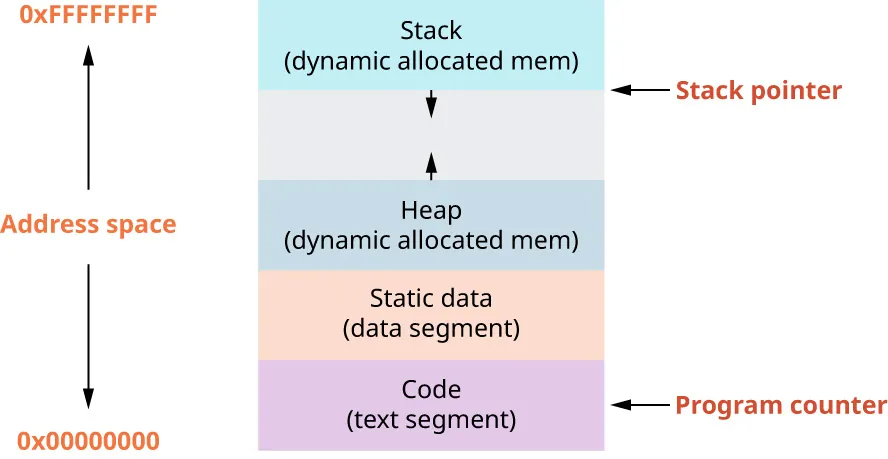
\includegraphics[width=0.5\textwidth]{image/Procesos.png}
    \caption{Espacio de direcciones de un proceso.}
  \end{figure}

  Los procesos son gestionados directamente por el sistema operativo,
  es el encargado de crear, programar y eliminarlos, no obstante, tambien un proceso 
  se puede comunicar con otro proceso, ya sea 
  en la misma máquina o en otra (cliente-servidor), 
  para esto se usan mecanismos de 
  comunicación entre procesos (IPC), 
  como tuberías, colas de mensajes, memoria compartida, etc.

  \newpage

  \section{¿Que es la imagen de un proceso?}

  La imagen de un proceso es la representacion 
  de varios elementos que conforman a un procesos que se esta ejecutando y que 
  tiene la informacion necesaria para que el sistema operativo pueda gestionarlo,
  estos elementos son, el programa ejecutable,
  los datos asociados al proceso (estado de los registros), el contexto de la ejecucion, los datos del usuario. 

  No obstante, la imagen del proceso tambien esta relacionado con la forma 
  en que el propio programa se organiza en memoria, 
  es por eso, que el espacio de direcciones del proceso tiene las siguientes 
  regiones: 
  \begin{enumerate}
    \item El segmento de texto contiene las instrucciones de máquina del programa. 
    \item El segmento de datos contiene datos estáticos inicializados y constantes.
    \item El segmento BSS contiene datos estáticos no inicializados.
  \end{enumerate}

  BSS: Es un área de memoria reservada para 
  aquellas variables no han sido inicializadas en tiempo de compilación y si en tiempo de ejecución. Su tamaño se conoce en tiempo de compilación y por eso size puede calcularlo.


  \thispagestyle{empty}
  
  % Impresión Referencias
  \nocite{*}
  \printbibliography[heading=bibintoc, title={Referencias}]
  
\end{document}